\chapter{Implementazione}
In questo capitolo si procede con l'implementazione del nuovo sistema, partendo dai design pattern seguiti per lo sviluppo. Si passa in seguito alla documentazione per definire quali API sono state sviluppate e in che modo sono state suddivise tra i servizi, procedendo con la presentazione dei framework utilizzati per la creazione dei componenti, mostrandone le relative parti di codice. Infine verrà mostrata la struttura del progetto e la sua suddivisione in moduli, e come questi comunicano tra loro.
\label{chap:implementation}

\section{Design Pattern}
\subsection{Inversion of Control}
L'\emph{Inversion of Control (IOC)} è il design pattern su cui si basano la maggior parte dei framework moderni: la sua implementazione è stata quindi indispensabile. Normalmente utilizzando una libreria è il nostro codice a richiamare gli elementi definiti all'interno di essa. Con l'introduzione di questo principio è il nostro codice ad essere richiamato dai componenti del framework, da qui il concetto di \emph{`inversione del controllo'}.

\subsubsection{Façade Pattern}
Questo design pattern contribuisce alla semplificazione delle interazioni con il framework o un set complesso di classi. Quando il codice lavora con un vasto set di oggetti appartenenti a librerie o framework sofisticati, normalmente è necessario inizializzare tali oggetti, tenere traccia delle loro dipendenze e chiamare i relativi metodi nel giusto ordine. In questo modo però il nostro sistema risulta strettamente legato all’implementazione di tali framework rendendolo difficile da mantenere. Il pattern risponde a questo problema. Una Facade è una classe che gestisce al posto nostro la logica appena descritta.

\paragraph{}Utilizziamo uno schema del sito \emph{Refactoring Guru} \cite{refactoring:facadepattern} per semplificare i concetti alla base del suo funzionamento. Prendendo come riferimento la figura [\ref{fig:facadepattern}] presentiamo gli elementi che lo compongono il pattern strutturale:

\begin{figure}[H]
    \centering
    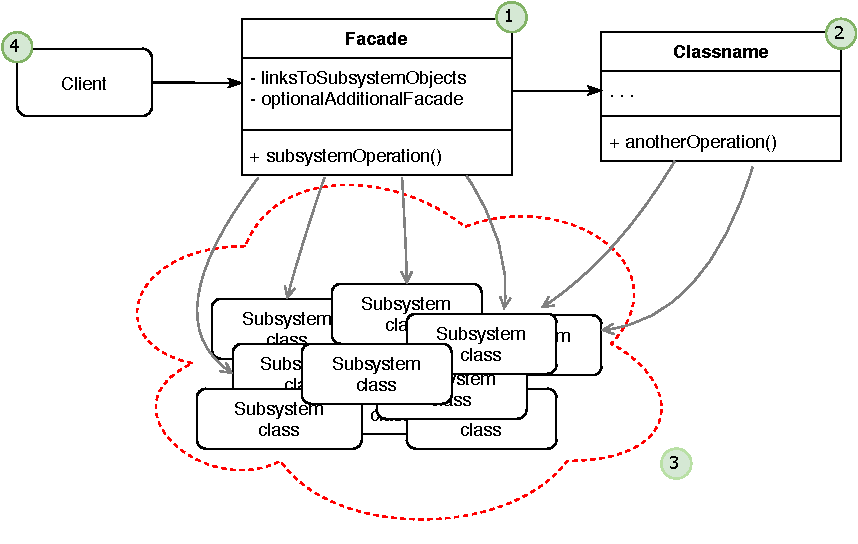
\includegraphics[width=0.75\textwidth]{images/03_1_facade_pattern.pdf}
    \caption{Componenti del Façade Pattern}
    \label{fig:facadepattern}
\end{figure}

\begin{enumerate}
    \item \textbf{Facade}: oggetto che dà accesso al set ristretto di funzionalità del Complex Subsystem
    \item \textbf{Additional Facade}: Facade aggiuntiva nel caso in cui si voglia tenere quella principale il più pulita e semplice possibile
    \item \textbf{Complex Subsytem}: libreria o framework complesso che vogliamo semplificare
    \item \textbf{Client}: Il client fa uso del Complex Subsystem attraverso la Facade
\end{enumerate}

%%%%%%%%%%%%%%%%%%%%%%%%%%%%%%%%%%%%%%%%%%%%%%%%%%%%%%%%%%%%%%%%%%%%%%%%%
\section{Documentazione}
La documentazione è stato il vero primo passo nel percorso di implementazione. Una decisione inusuale per lo sviluppo di un software, ma comprensibile per un caso di refactoring come questo, privo di una documentazione iniziale. 

%Sono state individuate un totale di 9 API da riscrivere, tutte originariamente sviluppate come metodi \emph{GET}. Di queste, 3 appartengono all'authentication server, mentre le restanti al booking server. Parte di queste API oltre alle operazioni sul database comprendono un sistema di notifica utente. Per queste API si è deciso di separare le due operazioni, delegando il sistema di notifica al \emph{Communication Server}.

\subsection{Swagger}
Swagger è un \emph{tool} composto da un set di software open source per progettare, creare e documentare \emph{RESTful APIs} attraverso l’\emph{OpenAPI Specification}, un formato di descrizione apposito per le REST APIs. In particolare aiuta a descrivere:
\begin{enumerate}
    \item \emph{endpoint} presenti e \emph{operazioni CRUD} che è possibile fare su di essi
    \item \emph{parametri} di input e output per ciascuna operazione
    \item metodi di \emph{autenticazione}
    \item informazioni relative al software, come contatti, licenza e termini di utilizzo
\end{enumerate}
Per descrivere il funzionamento del software si è utilizzato \emph{Swagger UI}, un tool che grazie all'uso delle \emph{annotazioni nel codice} e all'integrazione con il framework Spring permette di creare una pagina web dinamica che presenta tutte le informazioni relative alle API. Ciò che viene mostrato sulla pagina durante l'esecuzione corrisponde alla specifica delle API. Questo documento può essere anche scritto in YAML o JSON: il formato è facile da imparare e facilmente comprensibile sia dall'uomo che dalla macchina. 

\begin{figure}[H]
    \centering
    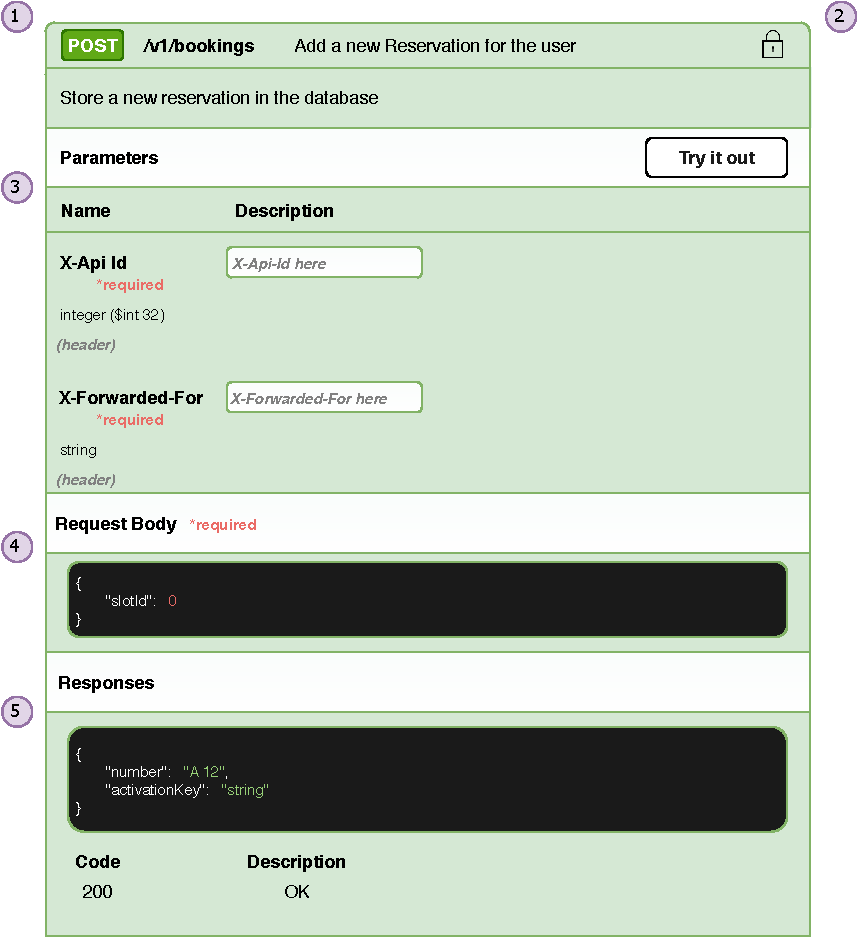
\includegraphics[width=0.85\textwidth]{images/03_2_swaggerui.pdf}
    \caption{Esempio di Specifica OpenAPI}
    \label{fig:swaggerexample}
\end{figure}

In figura [\ref{fig:swaggerexample}] viene presentato un esempio di specifica OpenAPI realizzata con swagger. Il documento descrive l'API di prenotazione di un servizio. In riferimento alla numerazione in figura, elenchiamo i campi che compongono la descrizione della nuova API.
\begin{enumerate}
    \item Metodo HTTP eseguito sull'url \emph{/v1/bookings} dove  \emph{`v1'}indica la versione delle attuali API. In questo campo e nel successivo è presente una breve descrizione dell'operazione.
    \item Il lucchetto in alto a destra, quando presente, indica che per quella chiamata è richiesta un'autorizzazione. In questo caso l'utente per poter prenotare un servizio deve aver effettuato l'accesso al sistema.
    \item In questo campo vengono descritti i parametri e gli header della chiamata. Per ogni parametro viene descritto il suo tipo, e viene aggiunta un informazione che avvisa nel caso questo sia obbligatorio. Di default in tutte le chiamate sono necessari due header: \emph{X-Api-Id} e \emph{X-Forwarded-For}. Il primo passa gli Id API della struttura, così che il sistema sappia sempre quali dati deve mostrare all'utente, mentre il secondo identifica il client che effettua la chiamata al server.
    \item Questa sezione descrive il body del messaggio, se presente. In questo caso la chiamata API viene fatta utilizzando il metodo POST, pertanto è previsto un oggetto JSON nel body della richiesta. L'utente per effettuare una prenotazione invia un oggetto contenente l'ID dello slot che vuole prenotare.
    \item Nel campo viene rappresentato l'oggetto JSON restituito nel caso la richiesta vada a buon fine. È possibile specificare anche altri codici di risposte che è possibile ricevere.
\end{enumerate}

%%%%%%%%%%%%%%%%%%%%%%%%%%%%%%%%%%%%%%%%%%%%%%%%%%%%%%%%%%%%%%%%%%%%%%%%%

%%%%%%%%%%%%%%%%%%%%%%%%%%%%%%%%%%%%%%%%%%%%%%%%%%%%%%%%%%%%%%%%%%%%%%%%%

%%%%%%%%%%%%%%%%%%%%%%%%%%%%%%%%%%%%%%%%%%%%%%%%%%%%%%%%%%%%%%%%%%%%%%%%%

%%%%%%%%%%%%%%%%%%%%%%%%%%%%%%%%%%%%%%%%%%%%%%%%%%%%%%%%%%%%%%%%%%%%%%%%%

%%%%%%%%%%%%%%%%%%%%%%%%%%%%%%%%%%%%%%%%%%%%%%%%%%%%%%%%%%%%%%%%%%%%%%%%%